
Validation of models is important to ascertain that the results are accurate. However, it should be noted that these long-term simulations are not predictions of the future, rather possible outcomes based upon certain assumptions. Therefore, the results from ElecSIM should be analysed by understanding the underlying assumptions of the model, and comparing inputs to outcomes.

Jager posits that a certain outcome or development path, captured by empirical data, might have developed in a completely different direction due to chance \cite{Jager2006a}. However, through observation, the processes that emerge from a model should be realistic and in keeping with expected behaviour \cite{Jager2006}.

We begin by comparing the price duration curve in the year 2018. Figure \ref{fig:price_duration_curve} shows the N2EX Day Ahead Auction Prices of the UK \cite{nordpool_2019}, the stochastic simulated electricity prices, and the non-stochastic electricity price throughout the year 2018.

It can be seen that adding stochasticity to fuel prices and variable operation \& maintenance improves accuracy of electricity prices in the initialisation year.


\begin{figure}[h]
	\begin{center}
		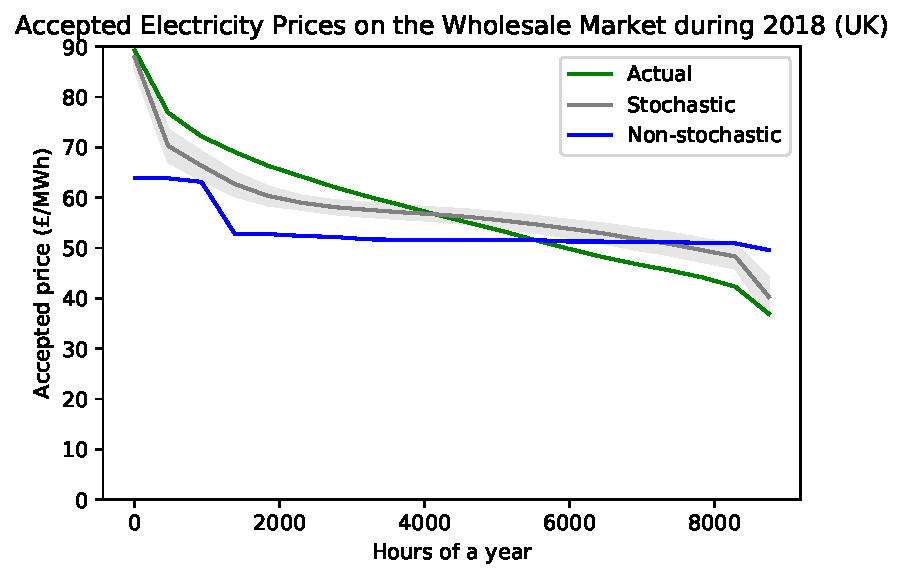
\includegraphics[width=0.5\textwidth]{figures/load_price_duration_curve_comparison.pdf}
		\caption{Price duration curve which compares real electricity prices to those paid in ElecSIM with stochasticity (40 runs) and no stochasticity.}
		\label{fig:price_duration_curve}
	\end{center}
\end{figure}

\begin{table}[h]
	\centering
	\csvautobooktabular{tables/validation/initialisation_run_validation.csv}
	\caption{Validation performance metrics.}
\end{table}



\begin{itemize}
	\item Validation of model 
	\begin{itemize}
		\item Compare price duration curve
		\item Compare power plant costs and NPV calculations
		\item Look number of steps ahead to compare electricity mix and compare to actual (cross-validation)
	\end{itemize} 
	\item Performance metrics - Comparison with EMLab, PowerACE (15 minute run time)
	\begin{itemize}
		\item Memory, disk size, runtime
		\item Increase in time complexity with additional data.
	\end{itemize}
\end{itemize}
